\documentclass{bigdata}
\usepackage[utf8]{inputenc}
\DeclareMathOperator*{\argmax}{arg\,max}
\DeclareMathOperator*{\argmin}{arg\,min}

\title{Multimedia Retrieval}
\author{Diego Renders (5740894) and Florian-Claudiu Gheorghica (6924123)}
\date{Oktober 2019}


\begin{document}
\maketitle

\section{Introduction}

\paragraph*{Problem statement.}

\newpage

\section{Part 1}

\subsection{File reading}

The files from the Princeton Shape Benchmark (PSB) were all provided in the OFF file format and an OFF reader was initially considered as a starting point. However, as a PLY format reader was likely to be necessary in the long-term, an OFF-to-PLY converter was written in order to enforce PLY as the default format for the application.
This converter simply creates a PLY header filled with data from the OFF file, then copies the vertex and face data over. While not a scalable approach for more complex OFF files, the converter was able to successfully process the entire PSB database.

\subsection{Database evaluation}
The database contains around 1800 models in OFF file format. All of the models contain only triangles as faces. The distribution of faces is shown in figure ?. The average number of vertices is 4221, the minimum 10, and the maximum 160940. The histogram, along with the average, shows that most of the models have a vertex count of smaller than twenty thousand. In order to successfully perform the upcoming steps of feature extraction the models need to have approximately the same number of vertices. Two actions can be undertaken to achieve this, supersampling and subsampling. Supersample the models with a low vertex count, and subsample the models with a large vertex count. A target number of vertices has to be chosen for this. One solution could be to choose the average. However because several of the meshes have a very high resolution (a hundred thousand vertices), subsampling this to reach the four thousand required vertices would ruin the original shape. Therefore the target vertices is chosen to be higher than the average, so that the higher resolution models retain their characteristics. The only downside for choosing a higher target number of vertices is an increase in computation time. The target number of vertices is set at forty thousand, and the methodology for supersampling and subsampling is explained in the following two sections.

\begin{figure}[h!]
  \centering
    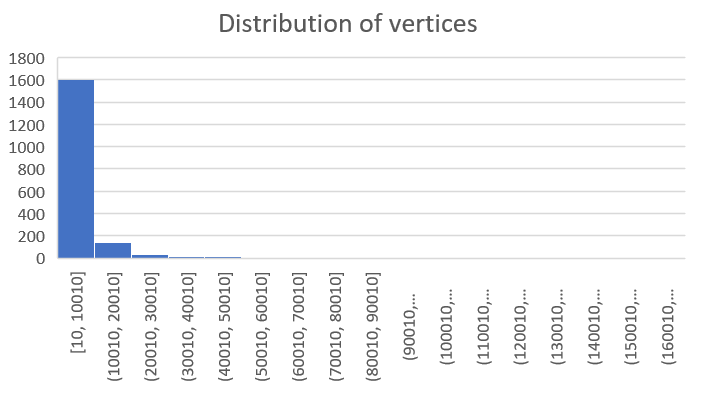
\includegraphics[width=\linewidth]{Pictures/verticesHist.png}
    \caption{Histogram showing the distribution of vertices in the PSB database}
\end{figure}

\subsection{Supersampling}
Supersampling is done in this implementation by splitting a larger triangle into 4 smaller ones via adding the midpoints of the original triangle’s edges as vertices and using them to form new triangles with the original vertices. An example is shown below:

\begin{figure}[h!]
  \centering
  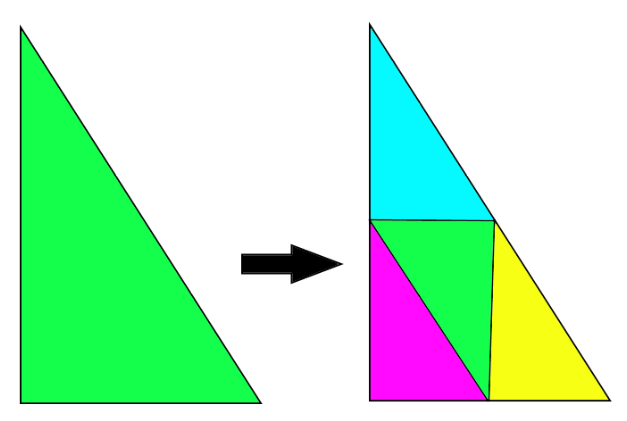
\includegraphics[width=\linewidth]{Pictures/triangle.png}
  \caption{Supersampling Example}
\end{figure}

To ensure the triangles obtained like this are not outliers in terms of their size, the cells in the model were first sorted by their area inside a vector, from smallest to largest. The area of each cell was calculated using the following formula:

\begin{equation}
S = \frac{|AB||AC|sin(\theta)}{2}
\end{equation}

Thus, at each step, only the triangle with the largest surface is split up into smaller triangles. The original triangle is removed from the vector, and the smaller triangles are inserted at positions that do not disturb the ordered property of the data structure.

\subsection{Subsampling}
For the task of subsampling the Polygon Mesh Processing (pmp) library is used. The SurfaceSimplification class is used to perform mesh decimation, taking as input the mesh and a target number of vertices. To demonstrate that this algorithm works correctly for our models a pre and post visualisation is shown in figure 2. This is the largest model in the dataset with 316.498 faces and 160.940 vertices. The post decimation model contains 78.473 faces and 40.000 vertices in the middle picture and 20.000 vertices in the right picture. Even though the model only has a fourth of its original vertices in the second case, it clearly retains its characteristics. And even when the vertex count is brought down to 20.000 vertices it is hard to distinguish them. Therefore we can conclude that the algorithm is a suitable tool for this project.

\begin{figure}[h!]
  \centering
  \begin{subfigure}[b]{0.3\linewidth}
    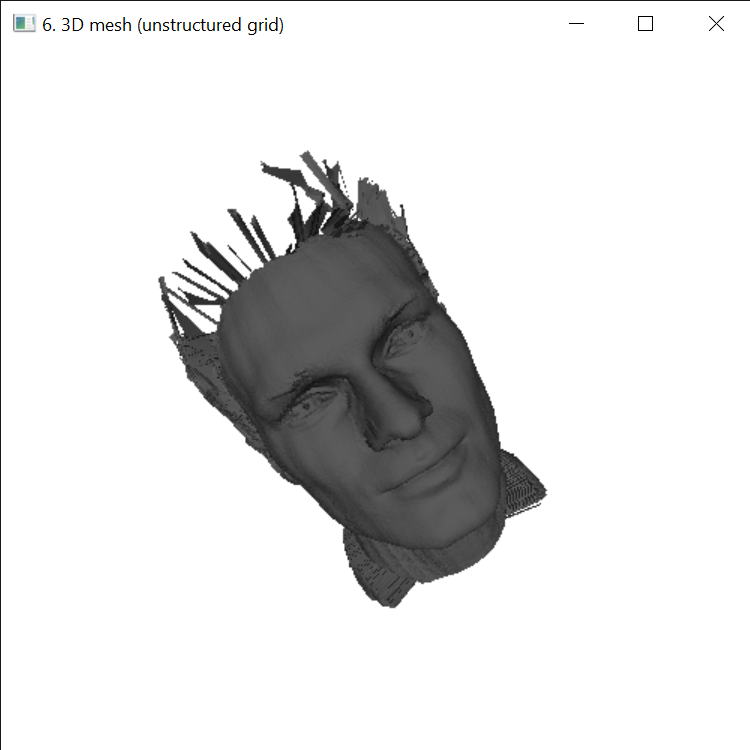
\includegraphics[width=\linewidth]{Pictures/preSub.png}
    \caption{160k vertices}
  \end{subfigure}
  \begin{subfigure}[b]{0.3\linewidth}
    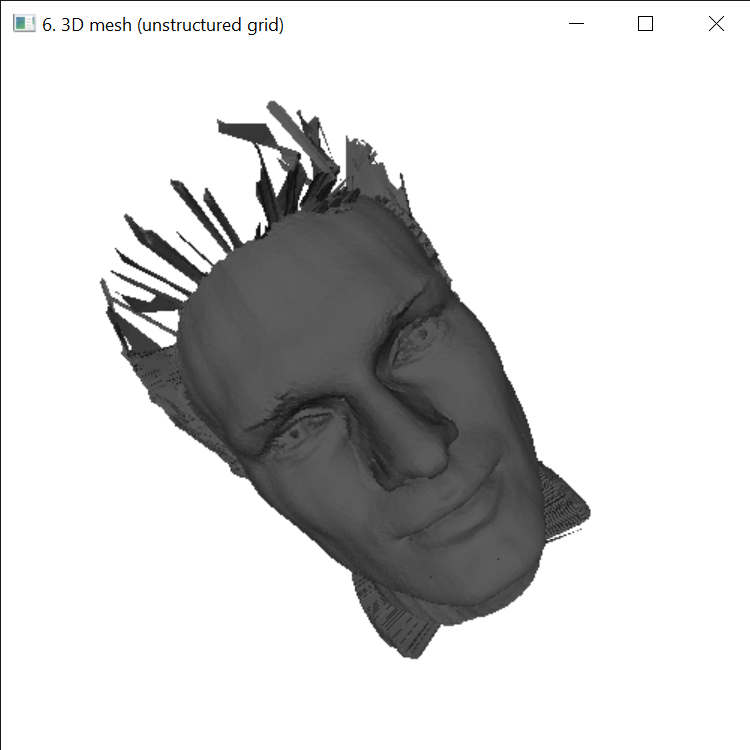
\includegraphics[width=\linewidth]{Pictures/postSub.png}
    \caption{40k vertices}
  \end{subfigure}
  \begin{subfigure}[b]{0.3\linewidth}
    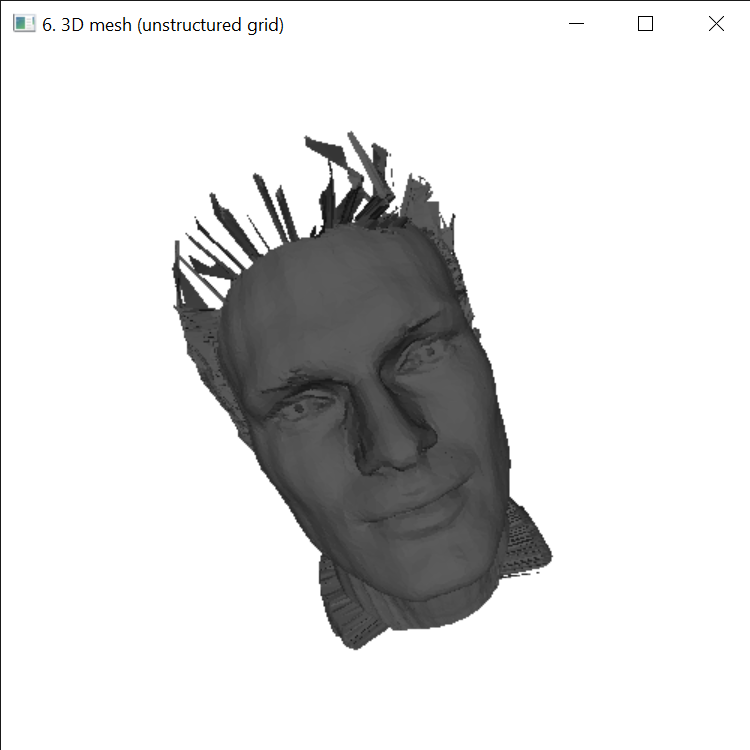
\includegraphics[width=\linewidth]{Pictures/postSub2.png}
    \caption{20k vertices}
  \end{subfigure}
  \caption{Results of mesh decimation for model m303}
  \label{fig:decimatedMesh}
\end{figure}

\subsection{Four step normalization}

Next each mesh will go through the four step normalization pipeline so that it is ready to be used in upcoming tasks. Figure 1 shows a visualization of what each step does, the red, green, and blue represent the $x$, $y$, and $z$ axises respectively from zero to one. The first step is to center on the Barycenter, than in step 2 PCA is done to orient the object in an intuitive way. Step 3 performs a fliptest which result in the majority of the mass in the object to be located in the negative side of the axis. Finally step 4 normalizes the model, which is excluded in the figure because the model was already normalized and thus would show no difference.

\begin{figure}[h!]
  \centering
  \begin{subfigure}[b]{0.4\linewidth}
    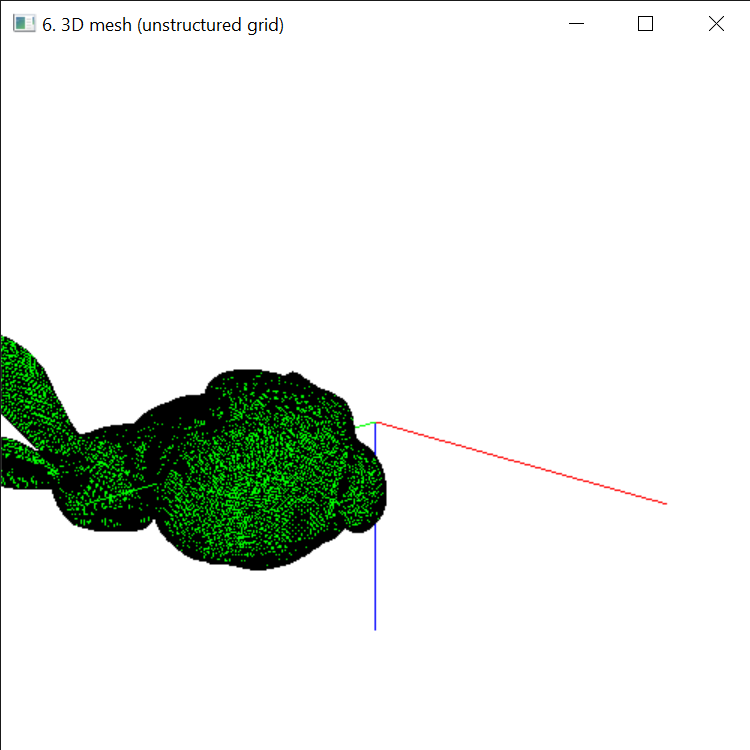
\includegraphics[width=\linewidth]{Pictures/Part2/Step0.png}
    \caption{Step 0}
  \end{subfigure}
  \begin{subfigure}[b]{0.4\linewidth}
    \includegraphics[width=\linewidth]{Pictures/Part2/step1.png}
    \caption{Step 1 Barycenter}
  \end{subfigure}
  \begin{subfigure}[b]{0.4\linewidth}
    \includegraphics[width=\linewidth]{Pictures/Part2/step2.png}
    \caption{Step 2 PCA}
  \end{subfigure}
  \begin{subfigure}[b]{0.4\linewidth}
    \includegraphics[width=\linewidth]{Pictures/Part2/step3.png}
    \caption{Step 3 Fliptest}
  \end{subfigure}
  \caption{Visualization of the Four step normalization pipeline.}
  \label{fig:bunny}
\end{figure}

\subsection{Step 1. Center on the barycenter}

For the first step the barycenter $b$ is calculated, which is the average x, y, and z coordinates of all vertices in the mesh. Next, each vertex $v$ is translated, by subtracting these averages from each of its points resulting in the new vertex position $u$.
\[
\begin{bmatrix}
u_x \\
u_y \\
u_z \\
\end{bmatrix}
=
\begin{bmatrix}
v_x \\
v_y \\
v_z \\
\end{bmatrix}
-
\begin{bmatrix}
b_x \\
b_y \\
b_z \\
\end{bmatrix}
\]

The result can be verified by calculating the average coordinates again, which should be 0 after the normalization.

\subsection{Step 2. PCA}
Prinicipal component analysis is done using the arglib library. The three eigenvectors $e_1$, $e_2$, and $e_3$ are returned by the algorithm. A translation matrix M is than created using the vectors $x$, $y$, and $z$, that represent the axises of the normal coordinate system.

\[
x = 
\begin{bmatrix}
1 \\
0 \\
0 \\
\end{bmatrix}
y =
\begin{bmatrix}
0 \\
1 \\
0 \\
\end{bmatrix}
z =
\begin{bmatrix}
0 \\
0 \\
1 \\
\end{bmatrix}
M =
\begin{bmatrix}
x \cdot e_1 & x \cdot e_2 & x \cdot e_3 \\
y \cdot e_1 & y \cdot e_2 & y \cdot e_3 \\
z \cdot e_1 & z \cdot e_2 & z \cdot e_3 \\
\end{bmatrix}
\]

The new vertex $u$ is obtained by multiplying this matrix with the old vertex $v$.

\[
\begin{bmatrix}
u_x \\
u_y \\
u_z \\
\end{bmatrix}
=
M
\cdot
\begin{bmatrix}
v_x \\
v_y \\
v_z \\
\end{bmatrix}
\]

The result of the translation can easily be verified. Doing PCA again on the translated mesh returns three eigenvectors that now correspond with the $x$, $y$, and $z$ axis.

\subsection{Step 3. Fliptest}
The eigenvectors used for the translation in the previous step are unoriented and thus give no information about to which side the model should be directed. Using the fliptest it is ensured that the majority of the mass resides in the negative half-space. Mass in this case is not indicated by the number of the vertices but also takes momentum into consideration, i.e. vertices farther away from the origin have a higher weight. Three variables are introduced: $w_x$, $w_y$, and $w_z$ that indicate the total weight of each of three coordinates. 
\begin{equation}
w_i = \sum sign(C_{t,i})(C_{t,i})^2
\end{equation}
 where $C_{t,i}$ is the $i^{th}$ coordinate of triangle t ($i \in {x,y,z}$). The latter part of the summation gives coordinates far away from the origin an higher weight, while the former part gives it either a negative or positive weight. These values are than used for a new translation matrix $M$. Which flips the coordinates if necessary, in case the mesh is already properly oriented $M$ will simply be the identity matrix.
\[
M = 
\begin{bmatrix}
sign(w_x) & 0 & 0 \\
0 & sign(w_y) & 0 \\
0 & 0 & sign(w_z) \\
\end{bmatrix}
\]

\subsection{Step 4. Normalization}
The last step scales the model in the unit volume, i.e. it can fit in a unit cube. First the min and max of the $x$,$y$, and $z$ coordinates of the axis-aligned bounding box is found. Next the largest distance $\delta$ between the min and max of these coordinates is used for the scaling factor $s = \frac{1}{\delta}$. Finally each vertex $v$ is multiplied with this factor to obtain the new vertex $u$.

\[
\begin{bmatrix}
u_x \\
u_y \\
u_z \\
\end{bmatrix}
=
\begin{bmatrix}
v_x \\
v_y \\
v_z \\
\end{bmatrix}
\cdot s
\]

A visualization is excluded, however the effectiveness of this step can easily be verified by looking at the resulting bounding box of the model.

\newpage

\section{Part 1}

There are two different types of features used to describe the meshes. The first are scalar features which consist of a single float. And the second are the histogram features, which for a histogram with $n$ bins contain $n$ float values representing the fraction of values contained in each bin. 
For extracting the histogram features random numbers will be generated. This is done by using the c++ function rand(). For the features that require multiple random numbers it is possible to generate duplicates, which would create large outliers. Therefore the numbers are re-sampled if there are any duplicates. Furthermore for obtaining the values of the histograms 20.000 of these samples will be taken for all histogram features.
The definition of these features, and how they will be normalized is discussed in the following subsections.

\subsection{Surface area}
The surface area of the mesh is the sum of all the face areas. In the dataset all the faces are triangles, therefore the surface area is the sum of all these triangles. The area of a triangle is calculated using the $triangle_area$ function provide by the $pmp$ library. The area of a triangle $t$ with vertices $u$, $v$, and $w$ is defined as followed:
\begin{equation}
area(t) = 0.5 * N((t_v-t_u) \times (t_w-t_u))
\end{equation}
Where $N(x)$ is the Euclidean norm of a vector $x$. The surface area feature $F_{SA}$ for a given mesh $M$ is than
\begin{equation}
F_{SA}(M) = \sum\limits_{i} area(t_i).
\end{equation}
where $t_i$ is the ith triangle of mesh M. The minimum value this feature can have is 0, but it does not have a maximum.

\subsection{bounding box volume}
The bounding box of a mesh is a rectangle that can be represented as two points, the opposite corners $bot$ and $top$. The volume $V$ is easily calculated as the $width \dot length \dot height$
\[
bot =
\begin{bmatrix}
x_{min} \\
y_{min} \\
z_{min} \\
\end{bmatrix}
top =
\begin{bmatrix}
x_{max} \\
y_{max} \\
z_{max} \\
\end{bmatrix}
\]
\begin{equation}
V(bot,top) = (x_{max} - x_{min}) \cdot (y_{max}-y_{min}) \cdot (z_{max}-z_{min})
\end{equation}
The bounding box volume feature $F_{BBV}$ for a mesh $M$ with its bounding box opposite corners $M_{bot}$ and $M_{top}$ is
\begin{equation}
F_{BBV}(M) = V(M_{bot},M_{top})
\end{equation}
The minimum value a bounding box can have is 0 when the mesh has no faces, and 1 when the bounding box is equal to the unit cube.

\subsection{Eccentricity}
The eccentricity of a mesh the ratio of the biggest eigenvalue of the covariance matrix to the smallest. The alglib library is once again used to do PCA and obtain the eigenvalues of the shape covariance matrix. For the eigenvalues $e_1$, $e_2$, and $e_3$ where $e_1$ is the largest value and $e_3$ the smallest, the eccentricity is
\begin{equation}
F_{EC}(M) = M_{e_3} / M_{e_1}
\end{equation}
Where $M_{e_3}$ and $M_{e_1}$ are the smallest and largest eigenvectors of mesh $M$ respectively. This describes the relation between the biggest and smallest eigenvectors, or also between the number of points spread in the x direction and the z direction. An object like a sphere or a head will have a high eccentricity, because their vertices are not spread out in a single direction. The picture of the head in figure 5 has an eccentricity of 0.72, while the leopard on the right has an eccentricity of 0.03.

\begin{figure}[h!]
  \centering
  \begin{subfigure}[b]{0.4\linewidth}
    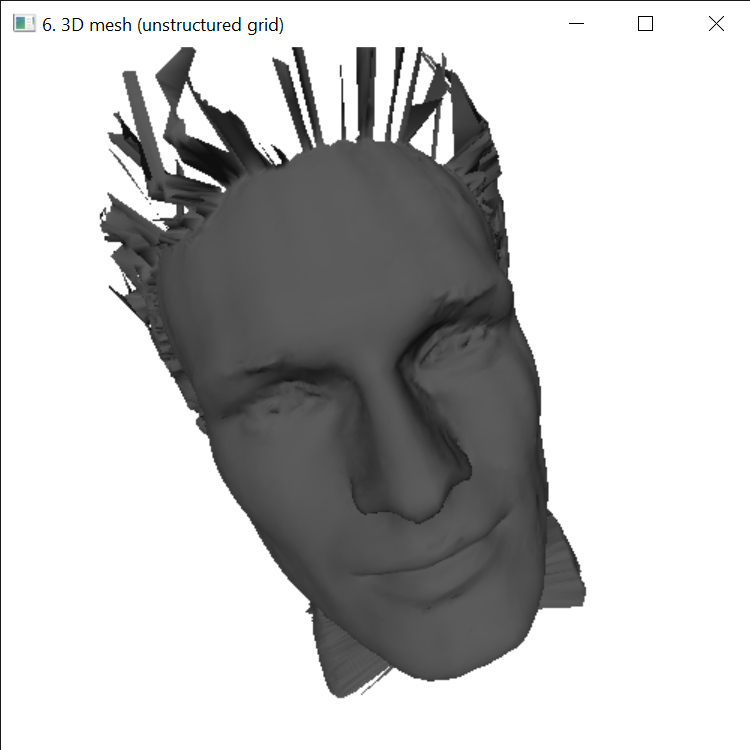
\includegraphics[width=\linewidth]{Pictures/Part3/eccHead.png}
    \caption{m303}
  \end{subfigure}
  \begin{subfigure}[b]{0.4\linewidth}
    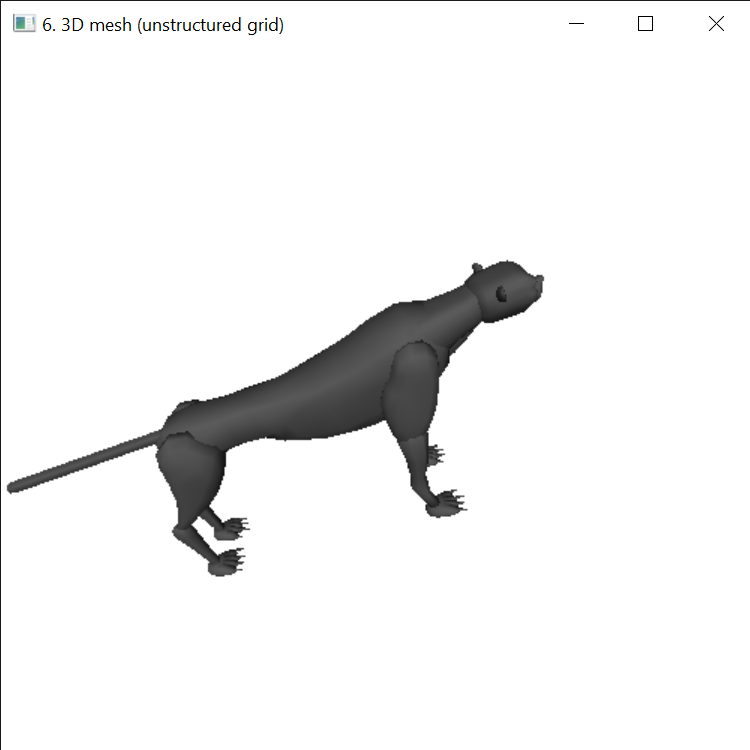
\includegraphics[width=\linewidth]{Pictures/Part3/eccLeo.png}
    \caption{m94}
  \end{subfigure}
  \caption{Two models with different eccentricity values}
  \label{fig:eccentricity}
\end{figure}
The eccentricity can go close to 0 for long objects or reach 1 for a perfect spherical form. Furthermore, this feature could also be extended to also describe the relation ratio between the other eigenvalues, $M_{e_2}$ / $M_{e_1}$ or $M_{e_3}$ / $M_{e_2}$.

\subsection{D1 - distance to barycenter}
This feature calculates the distance between a randomly generated point and the barycenter. The distance $D$ between two vectors $u$ and $v$ is calculated as follows
\begin{equation}
D(u,v) = \sqrt{\sum\limits_{i=1}^3 (u_i - v_i)^2}
\end{equation}
The minimum distance is obviously 0, and the maximum distance is equal to the diameter of a unit cube, $\sqrt{3}$, which is an unlikely scenario.

\subsection{D2 - distance between two points}
This time two random points are generated and the same distance function as for the D1 feature is used.
The min and maximum distances are the same as the previous feature.

\subsection{D3 - area of a random triangle}
To get a random triangle three random points are generated. The area of this triangle is calculated the same way as was done for calculating the total surface area. The square root of this value is than added to the histogram.
For the area of a triangle the minimum value is 0.

\subsection{D4 - are of a random tetrahedron}
Four random points $a$, $b$, $c$, and $d$ are generated that together will make the tetrahedron. The formula used for calculating the volume is:
\begin{equation}
V(a,b,c,d) = \frac{|(a - d) \cdot ((b - d) \times (c - d))|}{6}
\end{equation}

\subsection{A3 - angle between 3 random vertices}
The last histogram features uses three random points $u$, $v$, and $w$ to calculate the angle between them. These three points create a triangle that has three angles, however the order in which they are generated determines which angle is chosen. Therefore all three possible angles are calculates, and the maximum of those is chosen. For each angle the distance is chosen by using two vectors that share a similar point. For example, the vectors $a = v-u$ and $b = w-u$ give one possible angle of the triangle. The formula used for calculating an angle given two vectors is as follows:
\begin{equation}
Angle(a,b) = atan2(N(a \times b), (a \cdot b))
\end{equation}
Where N gives the euclidean norm of a vector, and atan2 the angle in the euclidean plane. The minimum value that the angle could be is 0, and the maximum is $\pi$.


\end{document}
